\artigotrue
\chapter{SPATIAL POINT PATTERN ANALYSIS OF SOIL SURVEY SAMPLING LOCATIONS}
\chapternote{This chapter is based on the studies \textit{An approach to help formalizing the purposive 
sampling strategy of classical soil surveys}, presented at the 20th World Congress of Soil Science 
\cite{Samuel-RosaEtAl2014b}, and \textit{Spatial point pattern analysis of soil survey sampling locations}, 
presented at the 10th European Conference on Geostatistics for Environmental Applications 
\cite{Samuel-RosaEtAl2014a}.}
\shorttitle{Spatial Pattern of Sampling Locations}
\label{chap:chap07}

%\def\ptkeys{Modelagem espacial do solo, Caminhamento livre, Análise de padrão pontual, Julgamento 
%especialista, Motivação}

%\begin{chapterabstract}{brazilian}{\ptkeys}
%Este é o resumo em português.
%\end{chapterabstract}

\def\enkeys{Soil spatial modelling. Free survey. Point pattern analysis. Expert judgement. Motivation}
  
\begin{chapterabstract}{english}{\enkeys}
Field soil spatial modellers usually select sampling locations based on tacit knowledge about soil-landscape 
relationships. The aim of this study was to assess the potential of point pattern analysis (PPA) to help 
understanding the purposive sampling strategy traditionally employed by field soil modellers. A dataset 
consisting of $n = 340$ soil samples obtained in a soil spatial modelling exercise carried out in Southern 
Brazil between \num{2008} and \num{2011} was used. PPA was performed using the 
\Rpackage{spatstat}. Soil sampling density was estimated using an isotropic Gaussian kernel smoother. The 
inhomogeneous G function and Monte Carlo simulations were used to evaluate the spatial pattern of the sampling 
points. A non-stationary Poisson point process model was fitted using covariates (land use and terrain 
attributes) and the sampling date to evaluate how environmental features and other intervening factors 
influenced the choice of sampling locations. Comparisons between PPA and judgements elicited from the 
soil modellers who carried out the soil modelling were used to validate the analysis. PPA showed that soil 
sampling locations are inhomogeneously distributed in the study area. Two areas were more densely sampled 
(nearest neighbour distances, $\text{NND} < \SI{125}{\m}$), one in the Southern sector, the other in the 
Middle-North-eastern sector. Sampling points have an approximately random spatial distribution in these two 
areas, while in the less densely sampled areas they are spaced at approximately regular distances ($\text{NND} 
> \SI{125}{\m}$). Land use, physiographic strata, and sampling date have a significant influence on the spatial
distribution of sampling locations. Land use yields the largest deviance reduction (\SI{6}{\percent}), followed
by sampling date (\SI{4}{\percent}) and physiographic strata (\SI{2}{\percent}). These results are in close 
agreement with judgements elicited from soil modellers. According to them, more densely sampled areas are 
those where they had a less consistent knowledge of soil-landscape relationships. These areas were visited in 
the first and last field campaigns, evidencing a temporal effect. On the other hand, most of the intermediate 
campaigns were carried out in areas where they had a better knowledge of soil-landscape relationships. Other 
intermediate campaigns were carried out in areas of poor accessibility, where soil modellers selected sampling 
locations by convenience. Intermediate field campaigns also coincided with a budget cut. The interplay of 
these intervening factors reduced the motivation of the soil modellers to conduct more intensive sampling. 
Soil modellers also reported that they performed a mental stratification of the study area prior to selecting 
sampling locations. Terrain features composed the first stratification variable, while land use was used as 
the stage-two stratification variable. The close agreement between PPA and judgements elicited from soil 
modellers suggests that PPA can help understand the sampling strategy used by soil modellers.
\end{chapterabstract}

\formatchapter

\section{INTRODUCTION}

Free survey has been successfully employed for many decades in soil spatial modelling. It is a model-based 
soil sampling method that relies on the mental model of soil-landscape relationships of field soil spatial 
modellers -- also known as soil surveyors. This mental model -- or tacit knowledge -- is built with the 
experience gained in the field and its quality generally is directly proportional to the years of field work. 
The main drawback is that formalising such complex models as verbal representations -- formal knowledge -- is 
rather difficult, the reason why it is rarely or only partially done. Thus, the tacit knowledge is at the risk 
of being lost when the soil modeller deceases, hindering the transmission of soil knowledge to young soil 
modellers. The present study assesses the potential of \emph{point pattern analysis} (PPA) as a tool to help 
understanding the purposive sampling strategy traditionally employed by field soil modellers.

The point pattern analysis toolbox includes multiple statistical techniques devoted to the analysis of sets of 
points distributed in the geographic space \cite{Diggle2003}. The main objective of these techniques is to 
provide empirical evidence to infer about the underlying process -- a biological or other deterministic 
mechanism -- that generated the \emph{point pattern} \cite{BivandEtAl2008}. A basic assumption is that the 
point pattern can be treated as a realization of a spatially homogeneous (stationary) random point process in 
the plane \cite{Diggle2003}. Assuming that soil observations made using the free survey method come from a 
stochastic process is unrealistic because soil observations are made following the conceptual model of 
pedogenesis of soil modellers. In other words, they are the product of an unspecified deterministic process, 
alike many other biological mechanisms evaluated using point pattern analysis. Point pattern analysis serves 
as an efficient exploratory tool in these circumstances and helps choosing non-stationary models to fit 
spatially inhomogeneous processes \cite{Baddeley2010} alike soil observation.

Calibrating a point process model requires some knowledge of the underlying process -- the biological 
mechanism -- that generated the point pattern. For example, such knowledge can be obtained by eliciting the 
judgements of experts, a common practice in many fields of research \cite{OHaganEtAl2006}. Usually, experts 
are consulted when important decisions have to be made during the development of a project or when there is 
great uncertainty about a phenomenon or event \cite{MeyerEtAl2001}. An expert is every individual who has a 
deep knowledge about a given theme. When trying to understand a soil observation process, an expert is every 
soil modeller that helped planning and conducting field sampling. The elicitation can be carried out in 
several ways \cite{Cooke1991, MeyerEtAl2001, OHaganEtAl2006} but due to operational issues, individual 
interview is the method most commonly employed. It also helps avoiding negative dominance effects due to 
eventual hierarchical relationships among experts \cite{Cooke1991}. Aggregation of expert judgements can be 
done using behavioural methods, where each expert evaluates the information provided by other experts until a 
common point is reached \cite{OrsiEtAl2011}.

Eliciting expert judgement is a key step towards understanding the underlying process that generated the point 
pattern of soil observation. Articulating expert information with psychological theories can provide important 
insights on the structure of this process. For example, it is agreed that the motivation to develop a series 
of tasks changes with time \cite{BonezziEtAl2011, Toure-TilleryEtAl2011a} and that the architecture of the 
surrounding environment influences the way space and distances are perceived \cite{Coeterier1994, 
EpsteinEtAl1998}. Taking such psychological elements into account could help explaining the origins of any
operational and conceptual tendencies noticed in the soil observation process as evidenced by the point 
pattern analysis and the interview of experts.

Environmental psychology is the field of science dedicated to the study of the relationships between human 
behaviour and the surrounding physical environment \cite{BonnesEtAl2002}. One of the recognized effects of the 
architecture of the surrounding physical environment on neurophysiological responses is the spatial enclosure 
\cite{EpsteinEtAl1998}. In natural landscapes, spatial enclosure expresses itself in environments surrounded by
elevated geomorphological features and rugged terrain such as in the valley bottom of mountainous regions. The 
effect of spatial enclosure on neurophysiological responses is complex \cite{StampsEtAl2004}, but it commonly 
results in the alteration of how distances are perceived \cite{Coeterier1994}. For instance, it can induce the 
perception that an enclosed space has a size larger than what it has in reality. A good example on how the 
perception of distances is altered due to spatial enclosure is the sensation of having walked hundreds of 
meters through a dense forest when only a few have been covered in reality.

Research on the psychology of goal pursuit and motivation has been carried out by many decades without coming 
to a common conclusion \cite{Toure-TilleryEtAl2011a, Hull1932}. Modern theories claim that there are motivation
shifts when a task involves the pursuit of multiple goals and describe it as the U-shaped motivation pattern of 
multi-goal pursuit \cite{BonezziEtAl2011, Toure-TilleryEtAl2011a}. In the beginning of a multi-goal project, 
motivation is high, and comes from the desire to accomplish all tasks using means that follow previously 
established rules. This is called the \emph{means-focused motivation}. With time the motivation to pursue the 
main goal decreases due to one or more factors such as diminished sense of goal achievability, decline 
of physiological and psychological resources (depletion) after first tasks are completed, positive goal-related 
emotions that reduce the efforts toward the main goal and shift the focus to another goal, and choosing to 
relax initial standards to save time and resources. The \emph{outcome-focused motivation} prevails in this 
phase, which is the bottom of the U-shaped motivation curve. As the main goal becomes closer, the motivation 
increases again from the desire to accomplish all tasks using means that follow previously established rules as 
in the beginning of the project. Stronger adherence to previously established rules and standards at the 
beginning and end of a project is possibly explained by the fact that the concerns about the image that one 
makes of himself (self-signalling concerns) usually are greater in these two phases of goal pursuit 
\cite{Toure-TilleryEtAl2011}.

\section{CASE STUDY}

A case study was conducted using a database composed of $n = 340$ soil observations made between \num{2008} 
and \num{2011} in a small catchment (\SI{20}{\km\squared}) located in the southern border of the Plateau of 
the Paraná Sedimentary Basin, in the city of Santa Maria, state of Rio Grande do Sul, Brazil 
(\autoref{fig:chap07-chap07-location}). Soil observations were made for the purpose of soil and land use 
mapping, as well as modelling soil carbon stocks and vulnerability to erosion \cite{Miguel2010, 
Samuel-Rosa2009, MouraBueno2012, Miguel2013}.

\begin{figure}[!ht]
\centering
\begin{minipage}{0.6\textwidth}
\subcaption{}
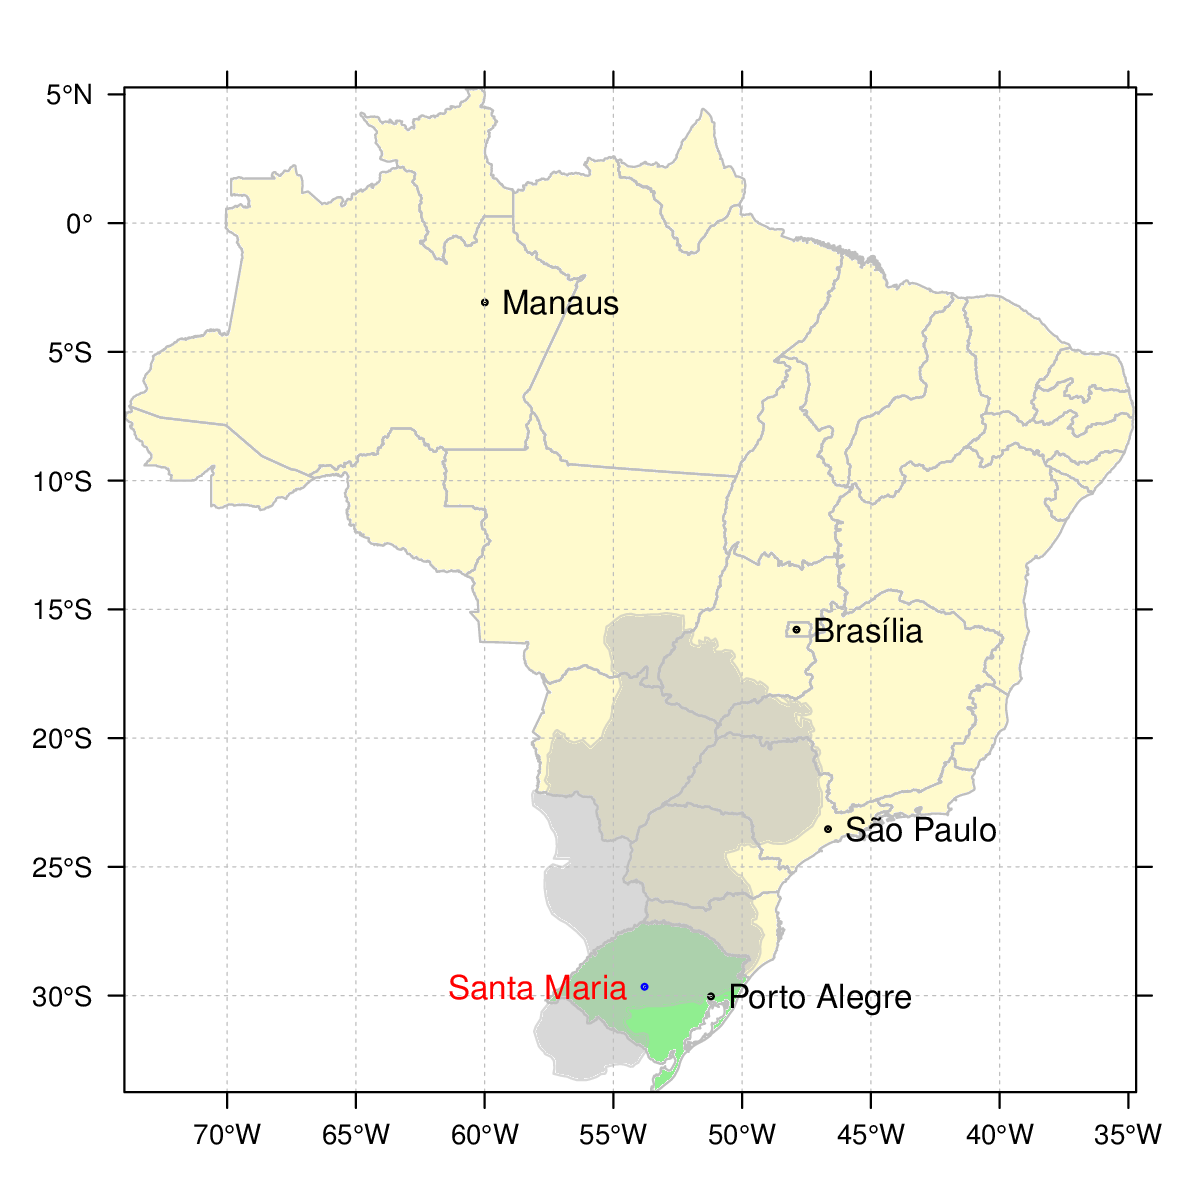
\includegraphics[width=\textwidth]{fig/chap07-location}
\end{minipage}
\begin{minipage}{0.6\textwidth}
\subcaption{}
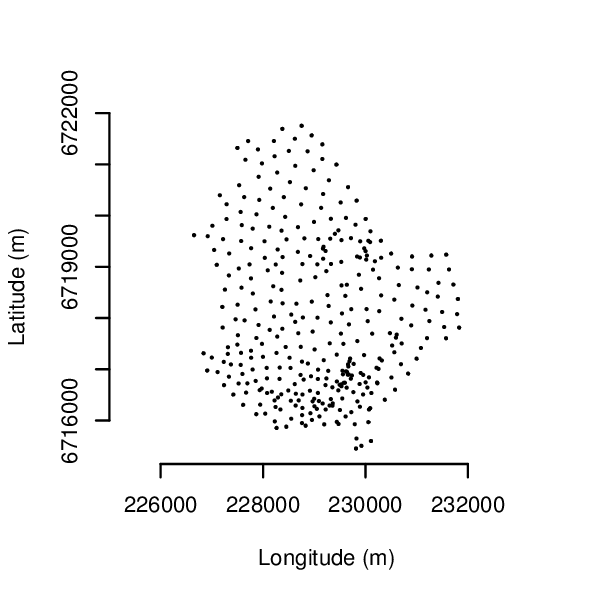
\includegraphics[width=\textwidth]{fig/chap07-ppp}
\end{minipage}
\caption[Location of the study area and the planar point pattern.]{Location of the study area (a) in the 
central region of the Southernmost Brazilian state, Rio Grande do Sul, and the planar point pattern (b) 
composed of $n = 340$ soil observations made between the years of \num{2008} and \num{2011}.}
\label{fig:chap07-chap07-location}
\end{figure}

Local climate is classified as Cfa (K{\"o}ppen climate classification -- subtropical humid without a dry 
season) with mean annual temperature of \SI{19.3}{\celsius}, and mean annual precipitation of \SI{1708}{\mm} 
well distributed throughout the year \cite{Maluf2000}. Relief varies between plain (slope between \num{0} and 
\SI{3}{\percent}) and mountainous (slope between \num{45} and \SI{100}{\percent}), and elevations range 
between \num{139} and \SI{475}{\m} above sea level. There are three main geological formations which consist 
of (a) basic, intermediate and acid igneous rocks (rhyolite-rhyodacite and andesite-basalt) of the Cretaceous 
period; (b) consolidated sedimentary rocks (aeolian and fluvial sandstones) of the Triassic and Jurassic 
periods; and (c) non-consolidated (fluvial and colluvial deposits) of the Quaternary period 
\cite{GasparettoEtAl1988, MacielFilho1990, Sartori2009}. Forest areas occupy more than half of the study area, 
followed by native grassland, shrubland, farmland, forestry, urban areas and artificial water bodies 
\cite{SamuelRosaEtAl2011a}.

\subsection{Elicitation of Expert Judgements}

Starting knowledge to understand the soil observation process was obtained eliciting the judgements of 
experts. An expert is every individual who has a deep, comprehensive knowledge about the object under study 
\cite{MeyerEtAl2001}, specifically, every soil modeller that helped planning and conducting the field 
campaigns that yielded the $n = 340$ soil observations in the study area. Due to operational constraints, the 
elicitation was carried out using email-based discussions and written narratives. First, written narratives 
were obtained by making a bibliographic review of published material such as articles, reports and theses. All 
information gathered was processed by the authors to yield a starting description of the soil observation 
process.

In the next step, field soil modellers were asked to prepare individual written description of the soil 
observation process. In their description, soil modellers were asked to point to the aspects that influenced 
most the selection of observation locations, as well as describe all important events and/or changes that 
might occurred in during the development of their project. Their description was then used to improve the 
existing description prepared by the authors, which was then submitted to appreciation by the field soil 
modellers. This step was carried out using a behavioural method \cite{OrsiEtAl2011}, specifically, email-based 
group discussions coordinated by the authors. These were responsible for aggregating expert judgements and 
continuously improving the description of the soil observation process until a common point was reached.

The resulting starting description of the soil observation process was used to define a set of covariates that 
could potentially be included in the point process model. These covariates are presented and described in 
\autoref{sec:chap07-elicited} along with a summary description of the soil observation process, while their 
use to construct the point process model is explained next in \autoref{sec:chap07-ppa}. 

\subsection{Point Pattern Analysis}
\label{sec:chap07-ppa}

Point pattern analysis was carried out using the \texttt{R}-package \texttt{spatstat} \cite{Baddeley2010}.

The first step consisted in estimating the observation window $W$, i.e. the limits of the spatial domain where 
soil observation were made. This was necessary because soil observation points are not constrained to the 
physical limits of the study area (\autoref{sec:chap04-sampling}). The estimate of $W$ was entirely based on 
the spatial point pattern assuming that the observation points have been generated independently and uniformly 
distributed inside an unknown $W$. The maximum likelihood estimate of the unknown $W$ is the rescaled convex 
hull $H'$ of the observation points, with the scaling factor equal to $1/\sqrt{1 - \frac m n}$, where $n$ is 
the number of observation points and $m$ the number of vertices of the convex hull $H$ \cite{RipleyEtAl1977}.

Spatial distribution of observation points was investigated using two measures of distance between observation 
points. The first is the \emph{empty space distance} or void distance, which measures the Euclidean distance 
from every single location in $W$ to the nearest existing observation point. The second is the 
\emph{nearest neighbour distance}, i.e. the Euclidean distance from every existing observation point to its 
nearest existing observation point. The latter was used to construct an \emph{Stienen diagram}, which consists 
of depicting every point using a circle with diameter and colour intensity proportional to its nearest 
neighbour distance. The Stienen diagram was visualised in Google Earth\rr{} to check for possible correlations 
between environmental conditions and nearest neighbour distances.

Evaluation of the spatial distribution of observation points suggested the observation intensity $\lambda$, 
i.e. the average density of observation points per unit area, to be spatially inhomogeneous. Contrary to the 
homogeneous case, where the intensity would be a function of the total number of observation points and the 
area of $W$, the inhomogeneous case requires estimating an \emph{intensity function} that accounts for the 
spatial variation of the intensity of the spatial point process. Here, the intensity function was estimated 
nonparametrically by kernel smoothing. Specifically, an isotropic Gaussian kernel with edge effect correction 
was employed, the bandwidth of the Gaussian kernel adjusted to minimize the square-mean-error criterion 
\cite{Diggle1985}.

The hypothesis that the spatial point pattern is completely random was tested comparing the fit between 
observed, $\widehat{G}$, and theoretical distribution functions of the nearest neighbour distance, $G$. For a 
spatial point pattern that conforms with the hypothesis of complete spatial randomness (CSR), the relation 
between observed and theoretical distribution functions of the nearest neighbour distance is approximately 
linear. Values $\widehat{G} > G$ suggest a clustered (aggregated) spatial point pattern, while values 
$\widehat{G} < G$ suggest a inhibited (regular) spatial point pattern. Monte Carlo simulations were used to 
assess the significance of departures from the theoretical distribution function. The simulation consisted of 
creating $s = 99$ independent realizations of a spatial point pattern with $n = 340$ observation points 
independently and identically distributed with inhomogeneous intensity on the observation window. Inhomogeneity 
was achieved using point estimates of observation intensity calculated with a leave-one-out Gaussian kernel 
smoother with edge effect correction \cite{BaddeleyEtAl2000}. The empirical distribution function of the 
nearest neighbour distance of all $s = 99$ realization were then used to compute the global upper and lower 
simulation envelopes. Here, we reject the null hypothesis of CSR if the observed distribution function of the 
nearest neighbour distance lies outside the envelope at any moment with an exact significance level $\alpha = 1 
/ (s + 1) = 1 / 100 = 0.01$.

Finally, assuming that the observation points have been generated independently of each other inside $W$, an 
inhomogeneous (non-stationary) Poisson point process model was calibrated to estimate the intensity function.
A series of spatially exhaustive covariates was used to define explanatory variables of the intensity 
function. These covariates served as proxies of the factors that determined the selection of observation 
locations by field soil spatial modellers. For that end, a generalized linear model with a log link was 
fitted by maximizing the pseudolikelihood using the Berman-Turner computational approximation 
\cite{Baddeley2010}. This spatial point process model was then used to estimate the intensity function to 
estimate the envelope of the detrended $G$ function.

\section{RESULTS}

\subsection{Elicited Expert Knowledge}
\label{sec:chap07-elicited}

According to the information gathered, the soil modellers had little experience with soil spatial 
modelling and this was the first time they were responsible for planning and making soil observations. Their 
expectation was to perform approximately $n = 500$ observations, given the available infrastructure, human 
resources and financial resources. The goal was to obtain a \q{satisfactory} coverage of both attribute and 
geographic spaces, with emphasis on the former. A mental stratification of the area was made to help achieve 
this goal. First, the area was divided into three strata according to geomorphological features: low elevation 
areas with flat and gently sloping terrain, steep slopes, and high elevation areas with gently sloping 
terrain. These strata represent three common physiographic regions of Southern Brazil called, respectively, 
Central (or Peripheral) Depression, Plateau Border and Plateau.

With their goal in mind, soil modellers started field campaigns in the Southern sector of the study area in 
\num{2008}. This area represents the Central Depression, were soil modellers had less knowledge of 
soil\-/landscape relationships. Access to most sampling sites was granted by the absence of geographic 
barriers and presence of a dense road network. After a few field campaigns, the soil modellers noticed that 
available resources and infrastructure would not allow visiting $n = 500$ sites. Access restrictions were 
imposed by some landowners and mean access time to observation locations was larger than expected. Besides, a 
budget shortage imposed important restrictions to the continuity of the study. As a consequence, the goal and 
planning of field campaigns had to be changed. The most sensible change was the decrease of observation 
intensity, requiring the approximate location of observation sites to be predefined beforehand at 
approximately equally spaced distances to obtain a satisfactory spatial coverage. A final outcome of at least 
$n = 300$ soil observations became the new focal goal of the soil modellers.

Next field campaigns took place in the steepest areas of the study area. These areas represent the Plateau 
Border and possess severe access restrictions due to strong slopes and dense forest cover. Access restrictions 
were again imposed by some landowners. Following, field campaigns were carried out in the Northern and 
North-eastern sectors of the study area. These areas represent the Plateau, where the soil modellers had a 
better knowledge of soil-landscape relationships. Overall, there were only minor access issues due to 
geographic barriers and very few restrictions were imposed by landowners. More field campaigns were carried 
out in the areas of the Plateau Border but avoiding difficult-to-access areas (steep slopes and dense forests).
In the last field campaigns, with a small amount of resources still available, the soil modellers performed a 
few more observations in some areas of the Plateau Border and Central Depression where their knowledge about 
the soil-landscape relationships was poorer. This yielded the final outcome of $n = 340$ soil observations.

\subsection{Point Pattern Analysis}

\subsubsection{Observation intensity}

The spatial distribution of the relative soil observation intensity estimated using an isotropic Gaussian 
kernel is shown in \autoref{fig:chap07-trend} (left plot). There are two regions where soil observation 
was more intense. The first and largest of them is located in the South-western sector, while the second is 
located in the Middle-North-eastern sector, with the largest values found in the South-western sector. 
Differences in observation intensity resulted in the occurrence of patches with poor geographic coverage 
(Figure \ref{fig:chap07-intensity}). The largest patches are located in the Middle and Middle-Eastern sectors.

\begin{figure}[!ht]
\centering
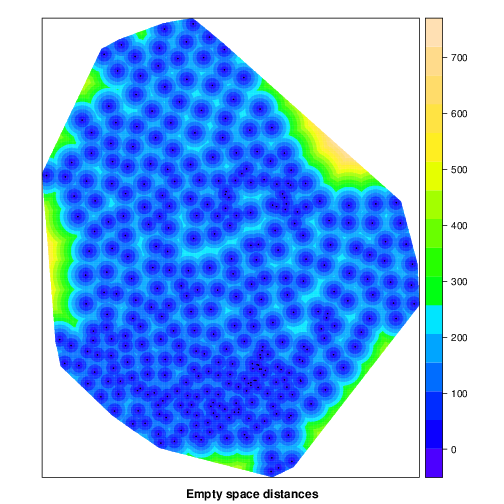
\includegraphics[width=0.6\textwidth]{fig/chap07-empty-space}
\caption[Estimated empty space distances.]{Estimated empty space distances. Values range from \num{1} to 
\SI{709}{\m}.}
\label{fig:chap07-intensity}
\end{figure}

The Stienen diagram (\href{https://www.dropbox.com/s/m00seobmpl5qtui/stienen.kml?dl=0}{click
here to download} and open in Google Earth\rr{}) helped identifying areas where the observation 
pattern is approximately regular, such as the Northern sector where the circles are approximately aligned and 
have about the same size. In the Southern sector, where the size of the circles is variable, the observation 
process seem to be approximately random. The relation between observation intensity and environmental features 
is also very clear. There is a strong relation between nearest neighbour distance and topography. Overall, the 
smallest nearest neighbour distance values seem to occur in the Central Depression and increase towards the 
Plateau Border (which has a dense forest cover) and the Plateau.

Observation intensity is also related to the temporal order in which observations were made 
(\autoref{fig:chap07-nndistG}). First observations were made at short distances, resulting in a higher 
observation intensity. With time, nearest neighbour distance started to increase. This increase occurred until 
about the \num{150}th soil sample, when the nearest neighbour distance reached about \SI{250}{\m} and 
remained approximately constant until the \num{300}th sample. After the \num{300}th observation, the 
nearest neighbour distance started to decrease and reached values around \SI{50}{\m}.

\begin{figure}[!ht]
\centering
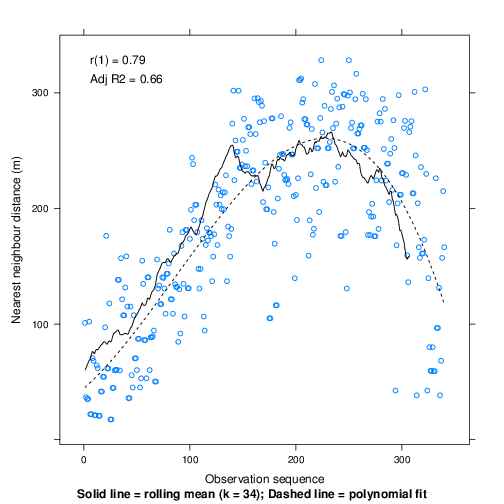
\includegraphics[trim=0mm 0mm 0mm 12mm, clip=true, width = 0.6\textwidth]{fig/chap07-nndistG}
\caption[Nearest neighbour distances and the order of soil observation.]{Estimated nearest neighbour distances 
(NND) as related to the temporal order in which soil observations were made. Twenty two field campaigns were 
carried out to make the $n = 340$ soil observations available. Deeper information about field campaigns is 
given in \autoref{fig:chap07-covars}. Function \texttt{rollmean} from \Rpackage{zoo} was used to estimate the 
rolling mean using a window of $n = 34$ points \cite{ZeileisEtAl2005}.}
\label{fig:chap07-nndistG}
\end{figure}

\subsubsection{Spatial distribution}

The estimated inhomogeneous \emph{G} function of the spatial distribution of the point process is shown in 
\autoref{fig:chap07-gest}. The curve of the empirical point process (continuous black line) follows a 
different pattern than the theoretical curve (dashed red line) of a completely random spatial point 
process. This result supports the initial understanding that the point pattern under analysis can be the 
realization of a deterministic process. \autoref{fig:chap07-gest} also shows the envelope of the estimated 
inhomogeneous \emph{G} function built with $n = 99$ Monte Carlo simulations. The global statistical 
test confirms that observations with a nearest neighbour distance smaller than about \SI{125}{\m} have a 
random pattern of spatial distribution. At nearest neighbour distances above \SI{125}{\m} the empirical curve 
shows a strong deviation from the envelope, indicating that the spatial distribution of the soil observations 
is approximately regular. Because there is a significant difference between the empirical and theoretical 
curves, the point process under analysis can be regarded as not being a realization of complete spatial 
randomness, but of an yet unspecified point process \cite{Baddeley2010}.

\begin{figure}[!ht]
\centering
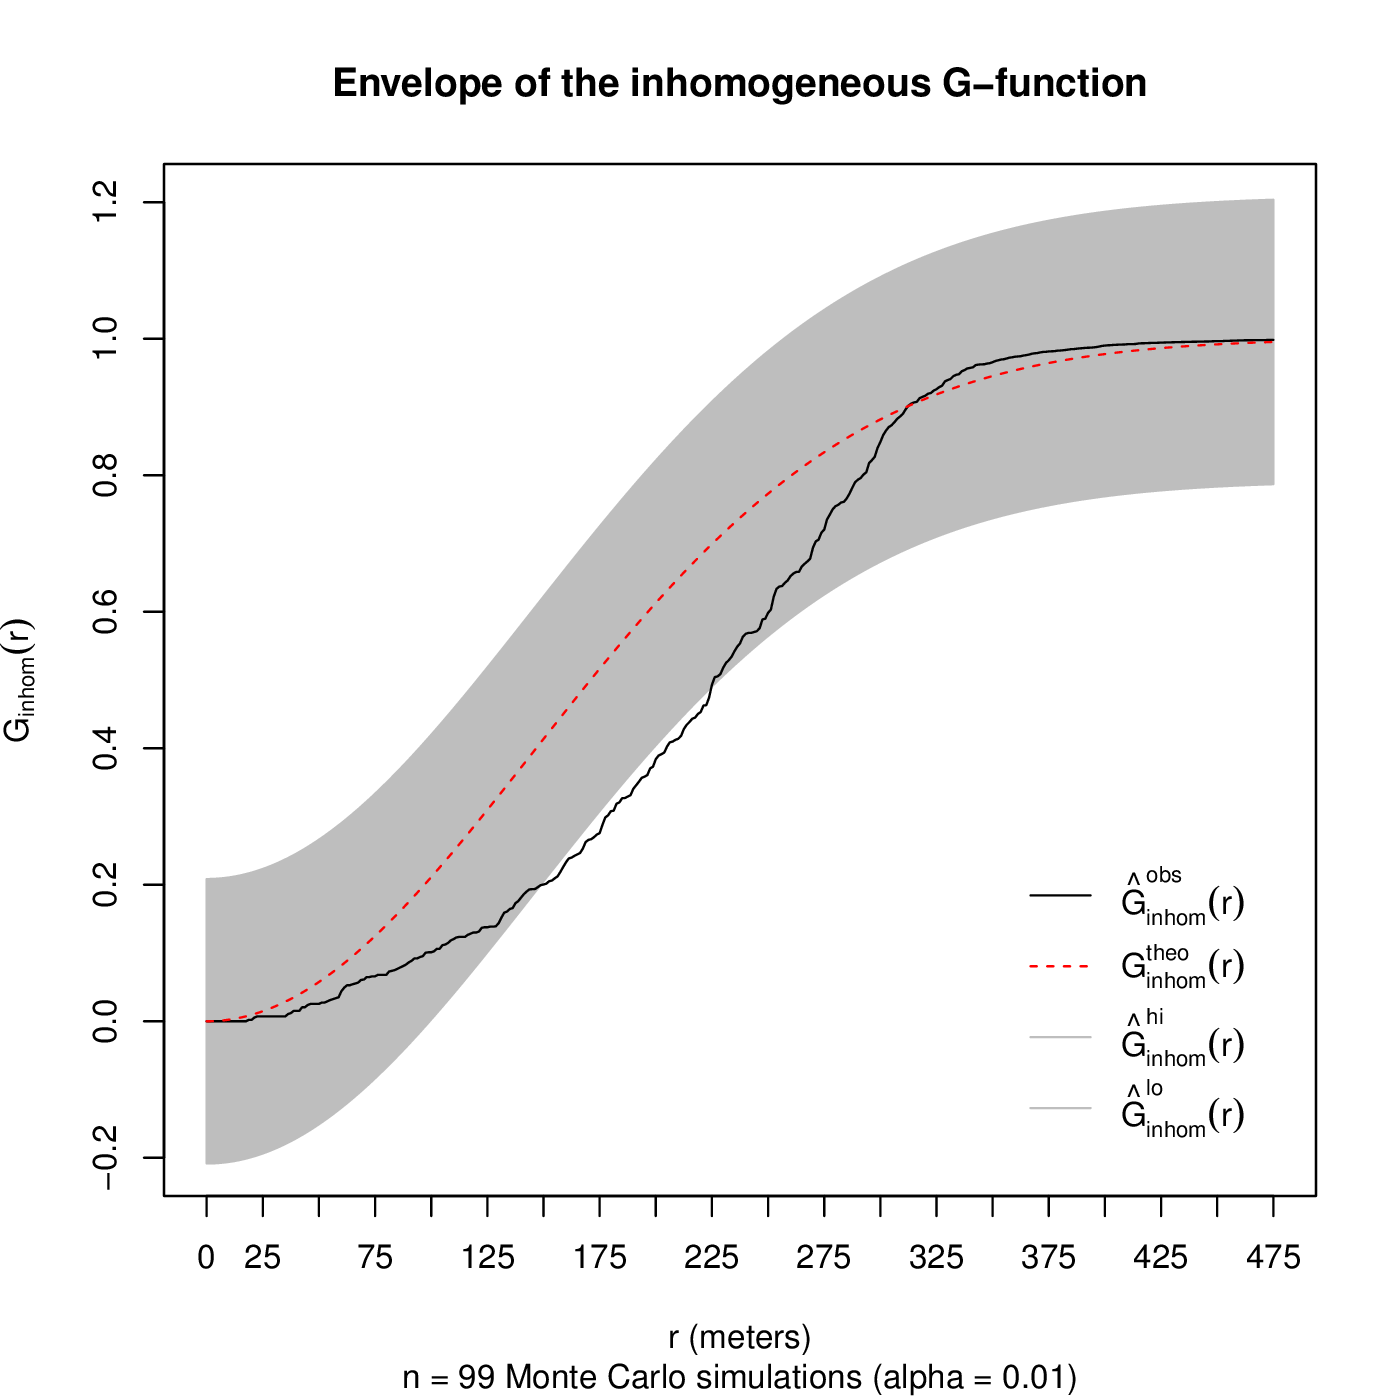
\includegraphics[trim=0mm 0mm 0mm 38mm, clip=true, width=0.6\textwidth]{fig/chap07-gest-sim}
\caption[Estimated inhomogeneous \emph{G} function and its global envelope.]{Spatial distribution of the planar 
point pattern estimated with the inhomogeneous \emph{G} function and its global envelope. Note that at NND 
smaller than about \SI{125}{\m} the point pattern can be regarded as having a random pattern of spatial 
distribution. These observations were made in first and last field campaigns as shown in 
\autoref{fig:chap07-nndistG}.}
\label{fig:chap07-gest}
\end{figure}

\subsubsection{Poisson point process model}

Three potentially explanatory covariates were suggested by the judgements elicited from the experts to be 
included in the Poisson model to explain the point pattern: land use (seven classes) 
\cite{SamuelRosaEtAl2011a}, terrain attributes derived from the sink-filled Shuttle Radar Topography Mission 
version \num{4} digital elevation model \cite{ReuterEtAl2007}, and field campaigns (indicator variables 
representing the 22 campaigns, respectively). The terrain attributes elevation, morphometric protection index 
and topographic position index were used to stratify the area into three physiographic strata, namely Central 
Depression, Plateau Border, and Plateau. A Dirichlet tessellation of the point pattern was computed to 
represent the field campaigns in the space domain.

Among all covariates available, land use, physiographic strata and field campaigns 
(\autoref{fig:chap07-covars}) are those which better explain the spatial distribution of the point process 
(\autoref{tab:chap07-deviance}). This corroborates the interpretation of the Stienen diagram (plotted in 
Google Earth\rr{}) and \autoref{fig:chap07-nndistG} made above. Land use produces the largest deviance 
reduction, followed by field campaigns and physiographic strata. The interactions between predictors also 
reduce the deviance and were not included in the model to avoid increasing its complexity.

\begin{figure}[!h]
\centering
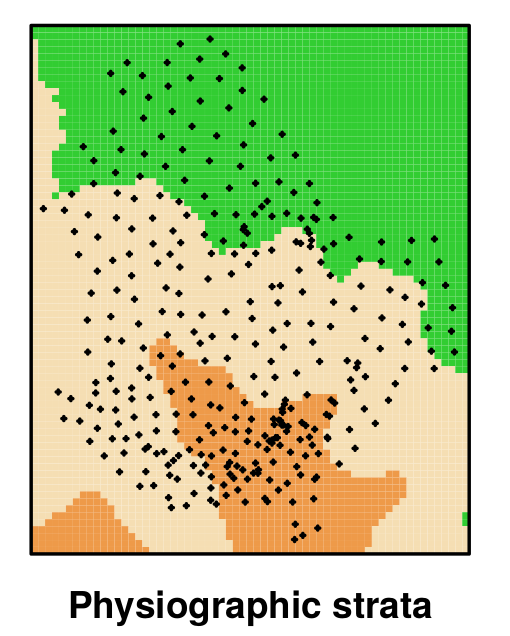
\includegraphics[width=0.32\textwidth]{fig/chap07-covarsA}
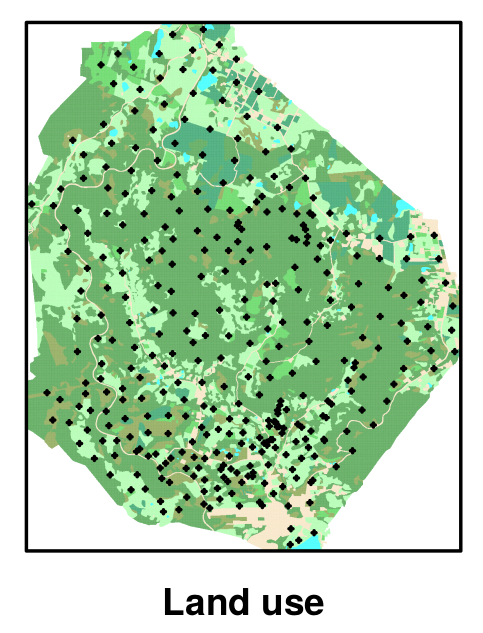
\includegraphics[width=0.305\textwidth]{fig/chap07-covarsB}
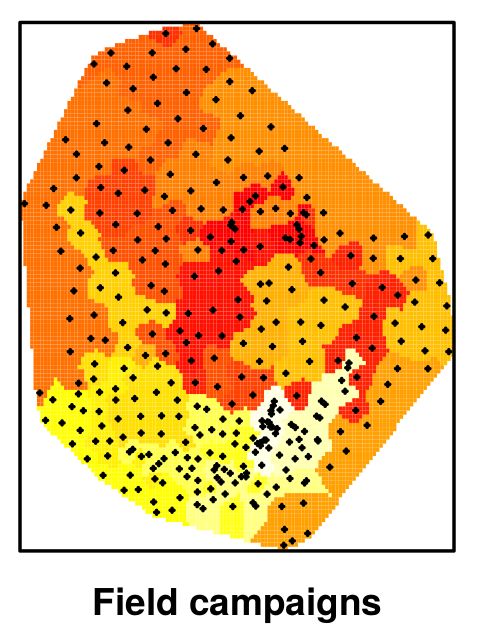
\includegraphics[width=0.3\textwidth]{fig/chap07-covarsC}
\caption[Covariates used to fit the non-stationary Poisson point process model.]{Covariates used to fit the 
non-stationary Poisson point process model superimposed with the planar point pattern. Physiographic strata 
include (South-North aligned): Central Depression, Plateau Border, and Plateau. Land use includes: native 
forest (more than \SI{50}{\percent} of the area), shrubland, animal husbandry, crop agriculture, forestry, 
urban, and water. Field campaigns has \num{22}~levels represented with increasing colour heat (white to red) 
from the first to the last campaign.}
\label{fig:chap07-covars}
\end{figure}

\ctable[
  caption  = {Analysis of deviance for the fitted non-stationary Poisson point process model with two-tailed 
  p-values for the chi-squared tests comparing the reduction in deviance due to the inclusion of each 
  predictor variable. Terms were added sequentially to the model (first to last).},
  cap      = {Analysis of deviance for the fitted non-stationary Poisson point process model.},
  label    = tab:chap07-deviance,
  notespar,
  pos      = !ht,
  maxwidth = \textwidth,
  % doinside = \scriptsize\setstretch{1.1},
  doinside = \small
  ]{lrrrrr}{
  }{ \FL
  Predictor		& Df	& Deviance	& Resid. Df	& Resid. Dev	& Pr($>$Chi)	\ML
  Intercept only	&  	&  		& 3240 		& 1943.05 	&  		\NN
  Physiographic strata	& 2 	& 38.03 	& 3238 		& 1905.03 	& 5.524e-09 	\NN
  Land use		& 6 	& 120.91 	& 3232 		& 1784.12 	& < 2.2e-16 	\NN
  Field campaigns	& 21 	& 63.28 	& 3211 		& 1720.84 	& 4.027e-06 	\LL
  }

Estimated coefficients for predictor variables show that observation intensity has a decreasing tendency in 
the Plateau Border and Plateau (\autoref{tab:chap07-coef}). The lowest observation intensity occurs in areas 
of native forests, urban land use and water bodies. All field observation campaigns were less intense than the 
first. Observation intensity reduction factor was similar between the second and seventh field campaigns 
(about \num{-0.75} times). The largest reduction occurred in the \num{13}th field campaign (\num{-2.18} 
times), when observation intensity started to increase again until the last field campaign.

\ctable[
  caption  = {Estimated coefficients for the fitted non-stationary Poisson point process model and their lower 
  and upper limits at the \SI{95}{\percent} confidence interval.},
  cap      = {Estimated coefficients for the fitted non-stationary Poisson point process model.},
  label    = tab:chap07-coef,
  notespar,
  pos      = !ht,
  maxwidth = \textwidth,
  % doinside = \scriptsize\setstretch{1.1},
  doinside = \small
  ]{lrrlrr}{
  \tnote[a]{Physiographic strata has three levels: Central Depression, Plateau Border and Plateau. Land use 
  has seven levels: native forest, shrubland, animal husbandry, crop agriculture, forestry, urban and water. 
  Field campaigns has \num{22} levels represented with increasing number from the first to the last campaign.
  
  \tnote[b]{Significance levels of the two-tailed Z test against the null hypothesis that each regression 
  coefficient is equal to zero are given for p-values of \num{0} (***), \num{0.001} (**), \num{0.01} (*), 
  \num{0.05} ( ) and \num{1} (na).}
  }
  }{ \FL
  Predictor\tmark[a,b] & Estimate & Standard error & Z test & Lower limit & Upper limit \ML
  (Intercept)		& -10.37 	& 0.24 			& na 	& -10.85	& -9.90         \NN
  Plateau border	& -0.03 	& 0.20 			&    	& -0.42 	& 0.37	\NN
  Plateau		& -0.07 	& 0.31 			&    	& -0.67 	& 0.53 	\NN
  Shrubland		& 1.17 		& 0.18 			& *** 	& 0.82 	        & 1.52 	\NN
  Animal husbandry	& 0.95 		& 0.14 			& *** 	& 0.67 		& 1.23 	\NN
  Crop agriculture	& 1.59 		& 0.19 			& *** 	& 1.22 		& 1.96 	\NN
  Forestry		& 1.10 		& 0.28 			& *** 	& 0.56 		& 1.64 	\NN
  Urban			& -1.12 	& 0.52 			& * 	& -2.13 	& -0.11 \NN
  Water			& 0.74 		& 0.72 			&    	& -0.68 	& 2.16 	\NN
  Field campaign 2	& -0.70 	& 0.32 			& * 	& -1.32 	& -0.08 \NN
  Field campaign 3	& -0.68 	& 0.31 			& * 	& -1.29 	& -0.07\NN 
  Field campaign 4	& -0.75 	& 0.32 			& * 	& -1.37 	& -0.13\NN
  Field campaign 5	& -0.85 	& 0.39 			& * 	& -1.60 	& -0.09 \NN 
  Field campaign 6	& -1.04 	& 0.37 			& **	& -1.77 	& -0.31 \NN
  Field campaign 7	& -0.74 	& 0.43 			&    	& -1.58 	& 0.09 	\NN
  Field campaign 8	& -1.36 	& 0.34 			& *** 	& -2.03 	& -0.69 \NN
  Field campaign 9	& -1.56 	& 0.43 			& *** 	& -2.40 	& -0.73 \NN
  Field campaign 10	& -1.49 	& 0.38 			& *** 	& -2.24 	& -0.75 \NN
  Field campaign 11	& -1.44 	& 0.41 			& *** 	& -2.24 	& -0.63 \NN
  Field campaign 12	& -1.39 	& 0.36 			& *** 	& -2.10 	& -0.68 \NN
  Field campaign 13	& -2.18 	& 0.44 			& *** 	& -3.04 	& -1.32 \NN
  Field campaign 14	& -1.64 	& 0.45 			& *** 	& -2.53 	& -0.75 \NN
  Field campaign 15	& -1.90 	& 0.36 			& *** 	& -2.61 	& -1.19 \NN
  Field campaign 16	& -1.93 	& 0.44 			& *** 	& -2.79 	& -1.07 \NN
  Field campaign 17	& -1.20 	& 0.38 			& ** 	& -1.94 	& -0.46 \NN
  Field campaign 18	& -1.25 	& 0.41			& ** 	& -2.06 	& -0.45 \NN
  Field campaign 19	& -1.14 	& 0.51 			& * 	& -2.15 	& -0.13 \NN
  Field campaign 20	& -1.33 	& 0.41 			& ** 	& -2.13 	& -0.53 \NN
  Field campaign 21	& -1.35 	& 0.38 			& *** 	& -2.10 	& -0.60 \NN
  Field campaign 22	& -0.28 	& 0.42 			&    	& -1.10 	& 0.54 	\LL
  }

The fitted non-stationary Poisson point process model gives a fine representation of the observation intensity 
estimated with the isotropic Gaussian kernel (\autoref{fig:chap07-trend}). Both sectors of high observation 
intensity are correctly predicted. However, relative intensity values are strongly over-predicted in the 
South-western sector, while in border areas they are strongly under-predicted. These under-predicted areas 
seem to be correlated to estimated empty space distances (\autoref{fig:chap07-intensity}).

\begin{figure}[!h]
\centering
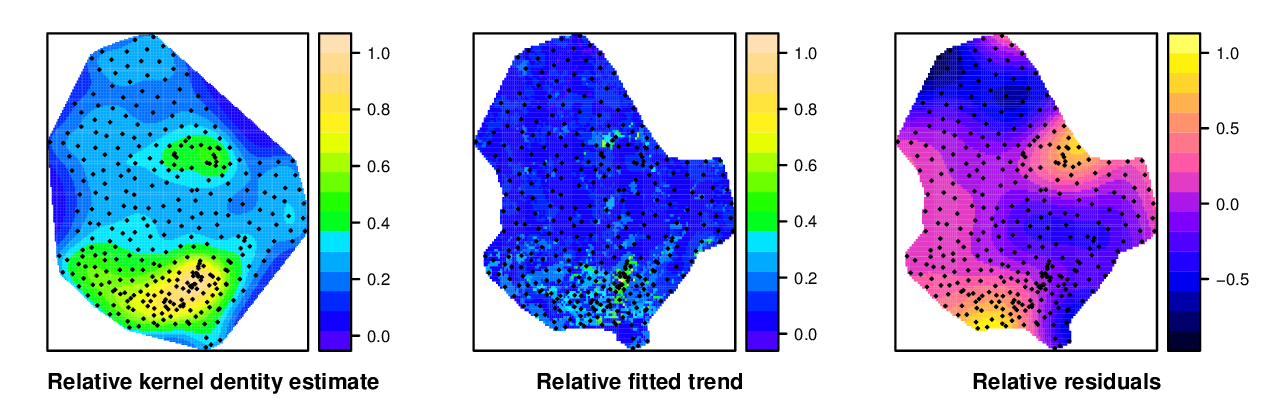
\includegraphics[width=\textwidth]{fig/chap07-kernel-trend-res}
\caption[Relative empirical kernel density estimate, and relative trend and residuals of the fitted 
non-stationary Poisson point process model.]{Relative empirical kernel density estimate (left), and relative 
trend (centre) and residuals (right) of the fitted non-stationary Poisson point process model. Data shown is 
relative to the largest absolute estimated value of intensity. Relative kernel density values range from 
\num{0.02} to \num{1.00}, relative trend values range from \num{0.01} to \num{1.00}, and relative residual 
values range from \num{-1} to \num{0.81}.}
\label{fig:chap07-trend}
\end{figure}

The envelope of the detrended estimated inhomogeneous \emph{G} function suggests that the fitted non-stationary 
Poisson point process model has efficiently captured the trend of the point pattern 
(\autoref{fig:chap07-detrended}). A slight difference between the curve of the empirical point process 
(continuous black line) and the theoretical curve (dashed red line) still exists in the middle range of the 
NND. Inclusion of interaction terms between predictors in the fitted model could help explaining this still 
remaining trend feature.

\begin{figure}[!h]
\centering
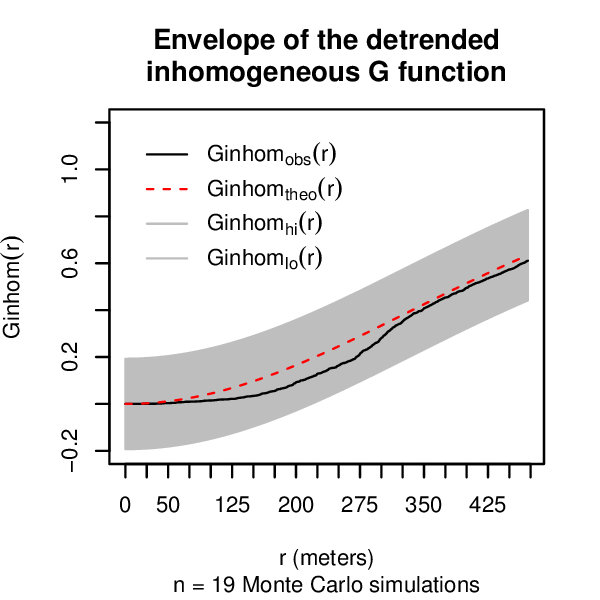
\includegraphics[trim=0mm 0mm 0mm 35mm, clip=true, width=0.6\textwidth]{fig/chap07-fit-gest-sim}
\caption[Global envelope of the detrended estimated inhomogeneous \emph{G} function.]{Global envelope of the 
detrended estimated inhomogeneous \emph{G} function. After detrending the curve of the empirical point process 
(continuous black line) follows a pattern similar to that of the theoretical curve (dashed red line) of a 
completely random spatial point process.}
\label{fig:chap07-detrended}
\end{figure}

\section{DISCUSSION}

The spatial distribution of the point process has features resulting from the influence of three key factors. 
The first is \textit{conceptual} and regards the knowledge of the soil modellers about soil-landscape 
relationships. The second factor is \textit{operational} and relates to the available infrastructure, human 
resources and budget to make soil observations, as well to access restrictions imposed by landowners and 
geographic barriers. The last factor is \textit{psychological}, which is also affected by the first two and is 
related to how the soil modellers perceive their surrounding environment and how the course of their 
motivation shifted during the soil observation process. The next three sections are devoted to better 
understand these factors.

\subsection{Concentrating on Problem Areas}
\label{subsec:chap07-conceptual}

Soil observations were made during studies organized by young soil modellers. Both soil modellers had just 
started their careers and had more experience with well drained, deep and high iron oxide content soils 
derived from igneous rocks and occurring on gently sloping to sloping relief. This is the same type of soil 
and relief that prevails in the Northern and North-eastern sectors of the study area. Because the soil 
modellers started the study using the free survey method, locating soil observations to test hypotheses 
posited according to their mental model of soil-landscape relationships, more observations were made on the so 
called \q{problem areas} \cite{Rossiter2000}. Problem areas are those areas for which the mental model of 
soil-landscape relationships is incomplete or possesses significant weaknesses, i.e. spatial soil variation is 
poorly predicted. Thus, it could be expected beforehand that the soil modellers would concentrate their 
efforts in Central Depression and Plateau Border areas. This is clearly evidenced by the higher observation 
intensity in the Central Depression and some areas of the Plateau Border, while the Plateau has a lower 
observation intensity.

\subsection{Managing Available Resources}

Field work is the main component of any soil mapping effort \cite{KempenEtAl2012}. Therefore, it demands an 
efficient planning of field campaigns to guarantee that the available infrastructure, human resources and 
budget are enough to accomplish the desired observation intensity. When the free survey method is used, 
planning of field campaigns strongly relies on the experience of the field soil modellers. Because the 
field soil modellers working in the study area had little field experience, it soon became clear to them
that field campaigns were inefficiently planned. Overall, the field soil modellers underestimated the costs of
variable components of field campaigns. One of these variable components is the access time to observation 
locations, which usually has a large impact on sampling costs \cite{DomburgEtAl1997}, especially in areas with 
many accessibility constraints.

Inefficient planning of field campaigns plus budget cuts and operational issues related to available 
infrastructure and human resources lead to the need for redefining the initially aimed total number of soil 
observations. Because the study started on problem areas, there is an \emph{operational} bias towards employing
stronger observation efforts in these areas, adding to the \emph{conceptual} effect described above (See 
\autoref{subsec:chap07-conceptual}). However, operational issues also lead to the reduction of the 
observation intensity on poorly accessible areas, such as those with steep slopes and dense forest cover of 
the Plateau Border. In classical sampling theory an observation process strongly influenced by accessibility 
issues is called \emph{convenience sampling} \cite{deGruijterEtAl2006}. The most extreme case occurs when soil 
observations are made only along the road network \cite{CambuleEtAl2013}. This is not the case of the 
observations made in the Plateau Border, but there is enough evidence to regard them as being the outcome of 
convenience sampling. Datasets obtained through convenience sampling usually present significant biases that 
affect the construction of robust soil mapping models \cite{BrusEtAl2011}. Therefore, it can be expected 
beforehand that most soil mapping models built for the study area will have a poor performance in the Plateau 
Border areas.

\subsection{Neurophysiological Responses}

\subsubsection{Spatial enclosure}

When making soil observations, enclosed places can be biasedly oversampled due to the effect of the spatial 
enclosure on the way that field soil modellers perceive the distances in their surrounding environment. If 
this hypothesis is correct, then it can be expected that the two soil modellers would have located soil 
observations at shorter distances in the Central Depression than in the Plateau, resulting in a denser soil 
observation in the former. The same explanation is valid for the denser soil observation made in the last field
campaigns carried out in a densely forested rugged terrain. Unfortunately the most expressive effect of the 
spatial enclosure occurs in the same places where the soil modellers had a poorer knowledge of soil-landscape 
relationships (Southern and Middle-Eastern sectors) and were not aware yet of the incompatibility between the 
available resources and their goals (Southern sector).

\subsubsection{Motivation shifts}

The U-shaped pattern of multi-goal pursuit shows a good fit to the soil observation process carried out by the 
field soil modellers in the study area. A strong motivation to follow well-known guidelines for soil 
observation existed in the first field campaigns. The soil modellers had the goal of obtaining a coverage of 
both attribute and geographic spaces to refine their knowledge of soil-landscape relationships and obtain a 
dataset that provided the means to make accurate predictions of the spatial variation of soil properties. 
Besides, this was one of the first studies under their complete responsibility, powering their initial 
motivational status. The possibility of understanding new soil-landscape relationships represented
a pleasant challenge for the young soil modellers. With time the soil modellers faced accessibility 
constraints that started depleting their physiological and psychological resources. The situation became worst 
when the soil modellers realized that the available resources and the initial goal were incompatible because 
the costs were underestimated and due to budget cuts. They were forced to shift their focus to the outcome, 
i.e. obtaining a \q{satisfactory} coverage of the geographic space while keeping the costs of the study 
below the available amount of resources available. In other words, they had to relax their initial standards 
to save resources (physiological, psychological and financial). The result was the reduction of the 
observation intensity. A new motivation shift occurred when the end of the project became closer and the soil 
modellers perceived that their resources were not completely depleted. Problem areas were visited again and 
the free survey method used to make new soil observations in a very similar way of the first field campaigns.

\subsection{Observation Model}

The approach presented here helped formalizing a verbal representation of the mental model of the soil 
scientists who produced the set of $n = 340$ soil observations in the study area. \autoref{fig:chap07-model} 
shows one of the possible ways of depicting this model. Nearest neighbour distance is used as a quantitative 
indicator of the progress of the observation process.

\begin{figure}[!h]
\centering
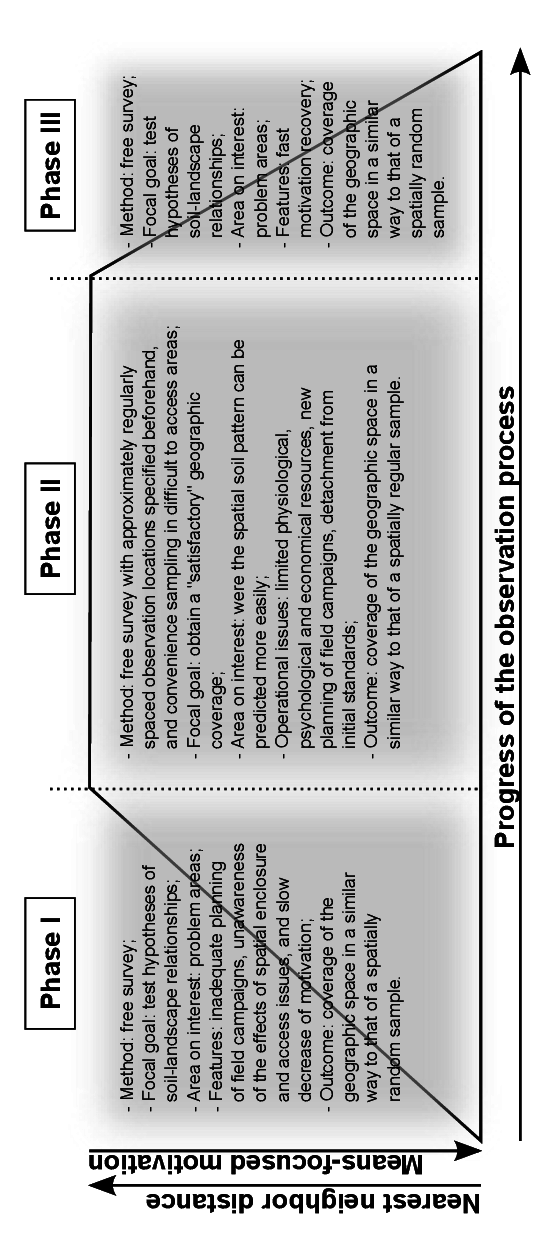
\includegraphics[width=70mm, angle=-90]{fig/chap07-observation-model}
 \caption[Theoretical model of soil observation.]{Theoretical model of soil observation depicted using the 
proposed approach that includes elicitation of expert knowledge, point pattern analysis and articulation of 
psychological theories of perception and 
 motivation. Phases I, II and III are guided by, respectively, means-, outcome- and means-focused motivation.}
 \label{fig:chap07-model}
\end{figure}

In the first phase the soil modellers employed the free survey method in its strict sense. The area was 
stratified into three primary observation units (physiographic strata) and many secondary observation units 
(land use type). The soil modellers were strongly motivated (means-focused motivation) and started observing 
the soil in problem areas. But they were unaware of the effects of spatial enclosure, access issues and of 
their inexperience which resulted in an inadequate planning of field campaigns. When the soil modellers became
aware of these effects (after a few field campaigns had been already carried out), the main goal of the 
project had to be reviewed and planning of field campaigns reformulated. This marks the end of the first phase 
of the observation model, which had as outcome a point pattern covering the geographic space in a fashion 
similar to that of a spatially random sample.

The second phase of the observation model starts when the soil modellers are consistently less motivated than 
when they started the observation process. This decreased motivation comes along with a new focal goal: making 
a minimum number of observations to obtain a \q{satisfactory} geographic coverage of the area. This is achieved 
by reformulating the planning of field campaigns. The free survey still is the observation method used but 
with the location of soil observations made beforehand at approximately equally spaced intervals. In the field 
the soil modellers are free to change this location according to their mental model of soil-landscape 
relationships but respecting the previously established spacing between observations. They also move from 
problem areas to those were the spatial soil pattern can be predicted more easily. When strong access issues 
are faced, convenience sampling is employed. The objective is to save physiological, psychological and 
financial resources. When the soil modellers realized that they had reached the new focal goal and that their
resources were not completely depleted yet, a new effort was employed to better understand problem areas. This 
marks the end of the second phase of the observation model, where the soil observation process was guided by an
outcome-focused motivation. The outcome of this phase is a point pattern covering the geographic space in a 
similar way to that of a spatially regular sample.

The last phase of the observation model starts when the soil modellers have a renewed motivation to make soil 
observations in problem areas using the free survey method in its strict sense. Soil observations are made 
while there are resources available. Field campaigns are better planned now because the soil modellers have 
gained field experience. But the effects of spatial enclosure can still be present. The outcome of 
this phase is a point pattern which has similar features to that produced in the first phase, i.e. covers the 
geographic space in a fashion similar to that of a spatially random sample. The main difference is that the 
number observations made is smaller as was the amount of resources available.

\section{CONCLUSIONS}

Several factors influence how field soil spatial modellers decide upon where to place soil observation 
locations. These are of three types: conceptual, operational, and psychological. The first concerns the 
knowledge of the soil spatial modellers about soil-landscape relationships, and seems to be connected with the 
years of field experience. The second relates to the available resources (infrastructure, workforce, and 
budget) to make soil observations, as well with access restrictions imposed, for example, by landowners and 
geographic barriers. The third relates to how the soil modellers perceive their surrounding physical 
environment and how the course of their motivation shifts during the soil observation process. Point pattern 
analysis helped understanding that there is a trade-off between conceptual and operational factors, which 
determines how the motivation of field soil modellers shifts towards one or another focal goal. Depending on 
the focal goal, the resulting point pattern resembles a random (testing hypotheses of soil-landscape 
relationships -- means-focused motivation) or a regular (maximizing the number of observations -- 
outcome-focused motivation) spatial sample. Understanding the reasons behind the location of soil observations 
in free survey can help soil spatial modellers designing more efficient data-driven sampling strategies.

% the following will not be included in the text
% \subsection{Next step}
% 
% Every modelling exercise starts with the development of a conceptual model (a verbal representation) of the 
% reality under study. This step has been covered in the present paper. The next step constitutes developing a 
% mathematical representation of this conceptual model, i.e. translating the verbal representation of the 
% reality 
% into a set of possible mathematical representations. One alternative is to use \textit{Species Distribution 
% Models} (SDM). The basic assumption of SDM is that the spatial distribution of a phenomenon can be predicted 
% relating sites of known occurrence with environmental covariates available for the entire study area 
% \cite{HenglEtAl2009e, WartonEtAl2010, HijmansEtAl2013}. Its use to model the soil observation process is 
% possible because soil observation by means of the free survey method can be regarded as a biological 
% mechanism 
% that takes place at specific sites as a function of environmental features. This biological mechanism has 
% the 
% simple objective of obtaining a better knowledge of the environment (i.e., the mental model of 
% soil-landscape 
% relationships of the soil modeller) to make a better use of it and assure the maintenance of the 
% \textit{species} (i.e., soil) through time.
% 
% Similar to standard ecological studies, soil observation reports are composed by presence-only data, that 
% is, 
% they hardly include information about the sites where soil observations were not made. In general, the total 
% number of observed sites (including soil pits, road cuts, gullies, river banks, rock outcrops, bore holes, 
% and 
% many others) is larger than the recorded/published number of soil observations, since only soil data at modal 
% sites are usually
% reported by soil modellers. Besides, the observation window is hardly known because soil modellers make 
% observations outside the reality under study and also bring their experience from soil observations in other 
% areas. A common approach in SDM modelling to deal with presence-only data is to fit a model to predict the 
% areas where soil observations are not likely to be made. This model is then used to produce the so-called 
% \textit{pseudo-absence} data.
% 
% Once the mathematical representation of the observation model is available it can be used for scenario 
% simulation exercises. For example, subsets of soil observations of varying sizes could be generated to 
% simulate
% the observation process in different budget scenarios and evaluate the effect of calibration sample size on 
% the
% performance of digital soil mapping models. The structure of the SDM approach applied to such exercise can 
% be 
% as described below (items from \num{1} to \num{4} follow \citeonline{HenglEtAl2009e}, while item 5 follows 
% \citeonline{BrusEtAl2007a}):
% 
% \begin{enumerate}
%  \item Estimate observation density in the geographic space using a kernel smoother;
%  
%  \item Estimate observation density in the feature space using factor analysis;
%  
%  \item Generate pseudo-absence locations of soil observations;
%  
%  \item Fit a universal kriging model to density values in the geographic space using environmental covariates
%  selected by fitting a non-stationary Poisson point process model to the presence-only data;
% 
%  \item Select subsets of observations of varying sizes using spatial simulated annealing with the 
% minimization 
%  of the spatially averaged universal kriging variance as optimization criterion.
% \end{enumerate}
% 
% Using a universal kriging model as the mathematical representation of the soil observation process is an 
% attractive alternative because it allows making geostatistical simulations and spatially depicting 
% uncertainties.


